\chapter*{Нерешённые головоломки}

\epigraph{Человек не может учиться иначе, как двигаясь от известного к неизвестному.}{---Клод Бернар (1813---1878)}

Цитируя моего приятеля: «Нерешённая головоломка --- это что ещё за хрень такая?».
Действительно, невозможно узнать, есть ли у задачи изящное решение, пока оно не найдено.
Тем не менее, некоторые нерешённые задачи привлекают довольно много внимания, из-за красоты и простоты постановки, удивляя при этом тем, что решение не найдено.
Математики, особенно такие как и ваш автор, воспитанные в эрдёшовской традиции искать самое простое из неизвестного, часто бравируют такими задачами.
Соберите несколько таких фанатиков вместе, и вы слышите разговор типа такого:

«Вот что меня беспокоит; ты знаешь ответ?»

«На самом деле, я даже не уверен, что знаю ответ на этот более простой вопрос.»

«Вы шутите? \emph{Я} даже не знаю \emph{вот этого}!»

Конечно, следует различать нерешённую задачу и гипотезу, как например гипотезу Римана или P = NP;
гипотезы могут не иметь красивой и элементарной формулировки, но они важны и изучаются потому, что они возникают (часто как препятствия) в погоне за истиной.
Формулировка гипотезы часто требует «профессиональных» математических понятий (графы, группы, многообразия, преобразования, представления и тому подобное), которые не допускаются в задаче, хотя они могут подразумеваться или быть необходимыми в её решении.

Нерешённые задачи могут быть развлекательными, интригующими, даже гадкими.
Но они не должны быть важны, \emph{то есть нам пока не должно быть это известно}.
Конечно, каждая такая задача важна как пробел в нашем знании.
Решение нерешённой задачи может дать ценную, серьезную технику; или это может быть результатом применения какой-то очень глубокой математики, далеко выходящей за рамки этой книги.
Некоторые задачи ниже, как гипотеза Франкла и $3x+1$ дилемма, привлекли столько внимания, что можно обоснованно утверждать, что любое решение будет представлять огромный интерес независимо от его применимости в других областях.

Эти задачи представлены здесь для вашего развлечения и чтобы напомнить о том, как мало мы знаем.
Если даже одну из них кто-то решит, узнав про неё в этой книге, то это будет небольшое чудо.
Если вам кажется, что вы решили одну из них, то скорее всего вы ошибаетесь.
Воспользуйтесь приведенными ссылками, вашими профессиональными математическими друзьями и вашей любимой поисковой системой в интернете, чтобы узнать больше о других попытках решить задачу.
Скорее всего вы узнаете, что попали в известную ловушку и не опозоритесь на публике.

Если вы все еще считаете, что у вас есть настоящее решение, оно должно быть записано и отправлено в подходящий математический журнал.
Не отправляйте его мне: я не эксперт ни по одной из задач.

\medskip

В этой главе, конечно, не будет раздела решений, но мы продолжим формат формулировки сначала, а затем комментарии и ссылки.
Начнем с классики от Джона Конвея.
Удачи!


\subsection*{Ангел и Дьявол Конвея}

Ангел летает над бесконечной шахматной доской, и время от времени должен садиться на клетку.
Он может пролететь не более 1000 ходов короля, до очередного приземления.

Пока Ангел летит, Дьявол, живущий под доской, может уничтожить любую клетку по своему выбору.

Может ли Дьявол поймать Ангела?

\subsection*{$\bm{3x+1}$ дилемма}

Начиная с произвольного положительного целого числа, будем повторять следующее действие: если оно чётно, то сократим его вдвое, а если нечётно, утроим его и добавим 1.

Доказать, что в конце концов мы зациклимся; или даже сильнее, что вы в конечном итоге мы придём к циклу $1, 4, 2, 1, 4, 2,\dots$.

\subsection*{Самая длинная общая подпоследовательность}
Генерируются две случайные двоичные последовательности длиной $n$, причём каждая цифра определяется независимо и равна 1 с вероятностью $p$.
Пусть $C_p(n)$ есть длина самой длинной общей подпоследовательности в двух, и пусть $C_p$ есть предел отношения $C_p(n)/n$.

Вычислите $C_{\frac12}$ или, по крайней мере, докажите, что $C_{\frac12}<C_{p}$ при $p\ne\tfrac12$.

\subsection*{Квадратура озера}

Докажите, что каждая простая замкнутая кривая на плоскости содержит четвёрку точек в вершинах квадрата.

\subsection*{Одинокий бегун}

Бегуны  стартуют в одной точке и бегут круговой дорожке единичной длины;
каждый бежит с посоянной скоростью и скорости у всех различны.

Доказать, что каждый бегун в какой-то момент времени будет на расстоянии хотя бы $1/n$ от любого другого бегуна.

\subsection*{Разбор пар в корзинках}

$n$ корзинок составлены в ряд.
В $i$-той корзинке лежат два шара с номерами $n+1-i$.
За одну операцию разрешается поменять пару шаров в соседних корзинках.

Сколько операций необходимо для того, чтобы каждый шар попал в корзинку со своим номером?

\begin{figure}[h!]
\centering
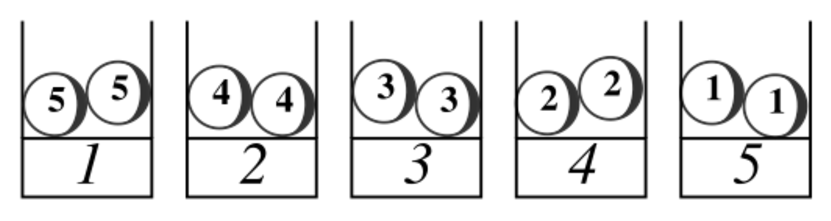
\includegraphics[scale=0.5]{Figs/UnsolvedPuzzles/bins}
\end{figure}

\subsection*{Развёртка многогранника}

Доказать, что произвольный выпуклый многогранник можно разрезать по рёбрам, так что полученная поверхность можно развернуть в плоский многоугольник.

\subsection*{Освещение многоугольника}

Любой ли многоугольник с зеркальными сторонами можно ли осветить одной лампочкой в некоторой его внутренней точке?

\subsection*{Треклы Конвея}

Треклом называют диаграмму на плоскости, состоящей из вершин и рёбер (кривые без самопересечений), такую что:
\begin{itemize}
\item каждое ребро начинается и заканчивается в двух различных вершинах, и не проходит через другие вершины; и
\item любая пара рёбер пересекает друг друга ровно один раз, либо в общей вершине, либо во внутренней точке.
\end{itemize}

Существует ли трекл с б\'{о}льшим числом рёбер, чем вершин?

\begin{figure}[h!]
\centering
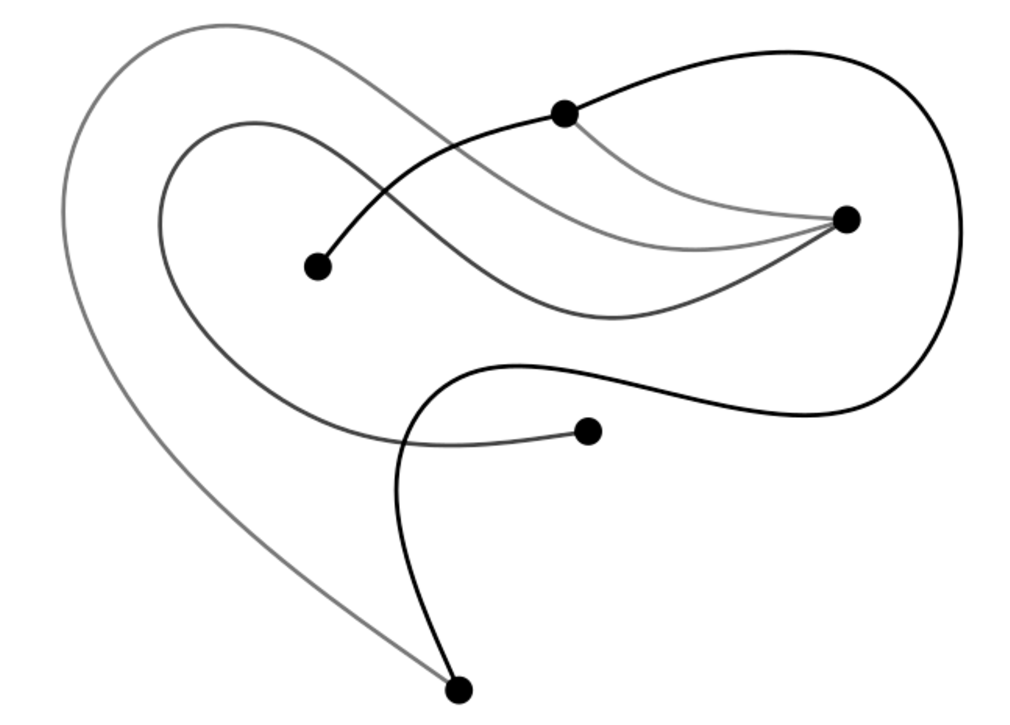
\includegraphics[scale=0.5]{Figs/UnsolvedPuzzles/thrack}
\end{figure}

\subsection*{Затор}

Вершины бесконечной решётки на плоскости выбираются независимо с вероятностью $p\in (0,1)$.
В каждую из выбранных вершин помещают автомобиль направленный либо на север либо на восток,
в каждом  случае направление выбирается независимо для подкидыванием монетки.

Движение регулируется светофорами, которые включают поочерёдно «зеленый-восточный» и «зеленый-северный».
При включённом зеленом-восточном, каждый восточный автомобиль, правая соседняя вершина от которого не занята, перемещается в эту вершину; остальные (в том числе заблокированные другим восточным автомобилем) остаются там, где они находились.

Когда включается зеленый-северный, каждый незаблокированный автомобиль в северном направлении перемещается на одну вершину в северном направлении.

Эксперименты говорят, что когда $p$ ниже определённого критического значения $p_0$,
автомобили постепенно разъезжаются.
Более того каждый автомобиль имеет предельную среднюю скорость, равную скорости автомобиля, который никогда не блокируется.
Но когда $p> p_0$ происходит обратное: автомобили попадают в безнадёжный затор, то есть каждый автомобиль делает только конечное число переездов, и останавливается навсегда.

Если вы готовы в это поверить, докажите одно из этих утверждений.

\subsection*{Гипотеза Мидлевелса}

Докажите, что вы можно обойти циклически все подмножества размера $n$ или $n+1$ в множестве размера $2n+1$, добавляя или удаляя один элемент за раз.

\subsection*{Построение диаграмма Венна}

Диаграмма Венна порядка $n$ представляет собой совокупность $n$ простых замкнутых кривых в плоскости, с трансверсальнымии пересечениями таких, что для любого набора кривых множество точек внутри кривых из набора, и снаружи остальных кривых является непустым связанной компонентой дополнения кривых в плоскости.

Можно ли расширить каждую диаграмму Венна  порядка $n$ до диаграммы Венна порядка $n+1$?

\subsection*{Стратегия для игры щёлк}

Число $k$ фиксируется, и Алиса и Боб играют в следующую игру.
Алиса называет делитель $k$.
Боб называет другой делитель $k$, который не кратен последнему числу названным Алисой.
Алиса называет третий делитель, который не является кратным ни одному из уже назаванных; 
и так далее.
Проигравает тот, кто называет 1.

Обратите внимание, что при $k=2^{n-1}3^{m-1}$, эта игра эквивалентна игре щёлк из предыдущей главы для плитки шоколада $m\times n$.
То же рассуждение показывает, что у Алисы существует выигрышная стратегия, но остаётся следующая задача, как для версии с шоколадкой, так и для приведённого обобщения:

Найдите выигрышную стратегию для Алисы!

\subsection*{Все дороги ведут в Рим}

Дана сеть (не обязательно плоская) городов и односторонних дорог со следующими свойствами:
из каждого города выходят ровно две дороги, и для некоторого фиксированного $n$, можно добраться из любого города в любой другой город пройдя по $n$ дорогам.

Докажите, что вы можно раскрасить дороги в красный и синий цвет таким образом, что (а) каждый город имеет выездную дорогу каждого цвета, и (б) есть набор инструкций (например, КССККСКССК), который всегда заканчивается в одном и том же городе, независимо от исходного города.

\subsection*{Круги в круге}

Докажите, что любой набор кругов с общей площадью $1$ можно упаковать в круг площади $2$.
А ещё лучше доказать, что в $d$-мерном пространстве любой набор из подобных копий выпуклого тела, с общим объёмом 1, можно упаковать в подобную копию объёма $2^{d-1}$.

\subsection*{Гипотеза Франкла}

Пусть $U$ --- конечное множество, а $T$ --- семейство непустых подмножеств $U$, которое замкнуто относительно объединения.
Докажите, что есть элемент в $U$, принадлежащий по меньшей мере в половине множеств в $T$.
